\documentclass[11pt,a4paper]{article}

% ========================================
% PACKAGES
% ========================================
\usepackage[utf8]{inputenc}
\usepackage[T1]{fontenc}
\usepackage{lmodern}  % Better font support for larger sizes
\usepackage[english]{babel}  % Change to your language
\usepackage[margin=2.5cm]{geometry}

% Mathematics
\usepackage{amsmath, amssymb, amsthm}
\usepackage{mathtools}

% Graphics and colors
\usepackage{graphicx}
\usepackage{xcolor}
\usepackage{tikz}
\usetikzlibrary{positioning, arrows.meta, shapes.geometric, calc, matrix}
\usepackage{pgfplots}
\pgfplotsset{compat=1.18}
\usepackage[most]{tcolorbox}

% Lists and formatting
\usepackage{enumitem}
\usepackage{parskip}
\usepackage{fancyhdr}

% Code listings (if needed)
\usepackage{listings}
\usepackage{algorithm}
\usepackage{algorithmic}

% CJK support for Chinese, Japanese, Korean characters
\usepackage{CJKutf8}

% Hyperlinks
\usepackage{hyperref}
\hypersetup{
    colorlinks=true,
    linkcolor=blue,
    urlcolor=blue,
    citecolor=blue
}

% ========================================
% THEOREM ENVIRONMENTS
% ========================================
\theoremstyle{definition}
\newtheorem{definition}{Definition}[section]
\newtheorem{example}{Example}[section]
\newtheorem{exercise}{Exercise}[section]

\theoremstyle{plain}
\newtheorem{theorem}{Theorem}[section]
\newtheorem{lemma}[theorem]{Lemma}
\newtheorem{proposition}[theorem]{Proposition}
\newtheorem{corollary}[theorem]{Corollary}

\theoremstyle{remark}
\newtheorem*{remark}{Remark}
\newtheorem*{observation}{Observation}

% ========================================
% CUSTOM COMMANDS
% ========================================
\newcommand{\R}{\mathbb{R}}
\newcommand{\N}{\mathbb{N}}
\newcommand{\Z}{\mathbb{Z}}
\newcommand{\Q}{\mathbb{Q}}
\newcommand{\C}{\mathbb{C}}

% ========================================
% HEADER AND FOOTER
% ========================================
\setlength{\headheight}{14pt}
\pagestyle{fancy}
\fancyhf{}
\lhead{\leftmark}
\rhead{nlp llm}
\cfoot{\thepage}
\renewcommand{\sectionmark}[1]{\markboth{#1}{}}

% ========================================
% TABLE OF CONTENTS DEPTH
% ========================================
\setcounter{tocdepth}{2} % Show only parts, sections, and subsections

% ========================================
% DOCUMENT INFORMATION
% ========================================
\title{\textbf{Natural Language Processing - LLM Module}\\
\large Artificial Intelligence}
\author{Jacopo Parretti}
\date{I Semester 2025-2026}

% ========================================
% DOCUMENT
% ========================================
\begin{document}

% Custom title page
\begin{titlepage}
    \begin{center}
        \vspace*{2cm}
        
        % University/Course info at top
        {\large\textsc{Artificial Intelligence}}
        
        \vspace{0.4cm}
        \textcolor{blue!60!black}{\rule{0.5\textwidth}{1pt}}
        
        \vspace{2.5cm}
        
        % Main title with modern spacing
        {\fontsize{36}{44}\selectfont\bfseries Natural Language Processing\\[0.5cm] LLM Module}
        
        \vspace{1.5cm}
        
        % Subtitle with clean design
        \begin{tcolorbox}[
            colback=blue!3!white,
            colframe=blue!40!black,
            width=0.6\textwidth,
            arc=1mm,
            boxrule=0.8pt,
            left=15pt,
            right=15pt,
            top=10pt,
            bottom=10pt
        ]
            \centering
            {\large\textit{Lecture Notes}}\\[0.3cm]
            \textcolor{gray}{Master's Program in Artificial Intelligence}
        \end{tcolorbox}
        
        \vfill
        
        % Clean course details
        \begin{tcolorbox}[
            enhanced,
            colback=white,
            colframe=gray!30,
            width=0.5\textwidth,
            arc=0mm,
            boxrule=0.5pt,
            left=20pt,
            right=20pt,
            top=12pt,
            bottom=12pt,
            shadow={2mm}{-2mm}{0mm}{black!10}
        ]
            \centering
            {\small\textcolor{gray!70}{\textbf{ACADEMIC YEAR}}}\\[0.4cm]
            {\Large 2025--2026}
        \end{tcolorbox}
        
        \vspace{2cm}
        
        % Author
        {\LARGE\textsc{Jacopo Parretti}}
        
        \vspace{1.5cm}
        
    \end{center}
\end{titlepage}

\newpage
\tableofcontents
\newpage


\part{Foundations of Neural Networks}

\section{Introduction to Neural Networks}

\subsection{The Concept of a Neuron}

Neural networks are computational models inspired by biological neural systems. At their core, they consist of interconnected units called \textbf{neurons} (or \textbf{nodes}).

\begin{tcolorbox}[colback=blue!5!white,colframe=blue!75!black,title=\textbf{Definition: Artificial Neuron}]
An \textbf{artificial neuron} is a mathematical function that:
\begin{enumerate}
    \item Receives multiple inputs $(x_1, x_2, \dots, x_n)$
    \item Computes a weighted sum of these inputs plus a bias term
    \item Applies an activation function to produce an output
\end{enumerate}
\end{tcolorbox}

\subsubsection{Mathematical Formulation}

The computation performed by a single neuron can be expressed as:

\[
z = \sum_{i=1}^{n} w_i x_i + b = w_1 x_1 + w_2 x_2 + \cdots + w_n x_n + b
\]

where:
\begin{itemize}
    \item $x_i$ are the input values
    \item $w_i$ are the \textbf{weights} associated with each input
    \item $b$ is the \textbf{bias} term
    \item $z$ is the weighted sum (also called the \textbf{pre-activation})
\end{itemize}

The final output of the neuron is obtained by applying an \textbf{activation function} $\sigma$ to the weighted sum:

\[
y = \sigma(z) = \sigma\left(\sum_{i=1}^{n} w_i x_i + b\right)
\]

\subsection{Activation Functions}

Activation functions introduce non-linearity into the network, enabling it to learn complex patterns. Common activation functions include:

\begin{tcolorbox}[colback=green!5!white,colframe=green!75!black,title=\textbf{Common Activation Functions}]
\textbf{1. Sigmoid:}
\[
\sigma(z) = \frac{1}{1 + e^{-z}}
\]
Outputs values in the range $(0, 1)$. Often used for binary classification.

\textbf{2. ReLU (Rectified Linear Unit):}
\[
\text{ReLU}(z) = \max(0, z)
\]
Outputs $z$ if $z > 0$, otherwise $0$. Most commonly used in modern deep learning.

\textbf{3. Tanh (Hyperbolic Tangent):}
\[
\tanh(z) = \frac{e^z - e^{-z}}{e^z + e^{-z}}
\]
Outputs values in the range $(-1, 1)$. Centers data around zero.
\end{tcolorbox}

\subsection{Multi-Layer Neural Networks}

The power of neural networks comes from connecting multiple neurons in \textbf{layers} to form deep architectures.

\begin{definition}[Feedforward Neural Network]
A \textbf{feedforward neural network} (also called a \textbf{multilayer perceptron}) consists of:
\begin{itemize}
    \item An \textbf{input layer}: receives the input features
    \item One or more \textbf{hidden layers}: perform intermediate computations
    \item An \textbf{output layer}: produces the final prediction
\end{itemize}
\end{definition}

\subsubsection{Architecture Visualization}

\begin{center}
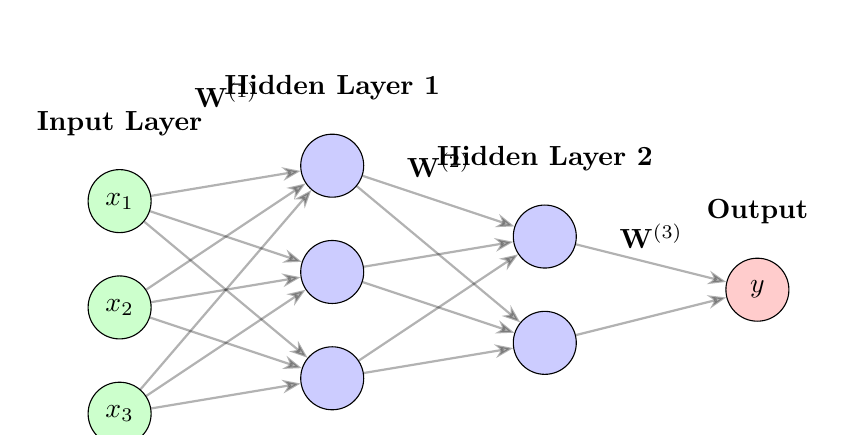
\begin{tikzpicture}[scale=0.9,
    neuron/.style={circle, draw, minimum size=0.8cm, fill=blue!20},
    input/.style={circle, draw, minimum size=0.8cm, fill=green!20},
    output/.style={circle, draw, minimum size=0.8cm, fill=red!20},
    arrow/.style={-Stealth, thick}
]

% Input layer
\node[input] (x1) at (0,3) {$x_1$};
\node[input] (x2) at (0,1.5) {$x_2$};
\node[input] (x3) at (0,0) {$x_3$};

% Hidden layer 1
\node[neuron] (h11) at (3,3.5) {};
\node[neuron] (h12) at (3,2) {};
\node[neuron] (h13) at (3,0.5) {};

% Hidden layer 2
\node[neuron] (h21) at (6,2.5) {};
\node[neuron] (h22) at (6,1) {};

% Output layer
\node[output] (y) at (9,1.75) {$y$};

% Connections from input to hidden layer 1
\foreach \i in {1,2,3}
    \foreach \j in {1,2,3}
        \draw[arrow, opacity=0.3] (x\i) -- (h1\j);

% Connections from hidden layer 1 to hidden layer 2
\foreach \i in {1,2,3}
    \foreach \j in {1,2}
        \draw[arrow, opacity=0.3] (h1\i) -- (h2\j);

% Connections from hidden layer 2 to output
\foreach \i in {1,2}
    \draw[arrow, opacity=0.3] (h2\i) -- (y);

% Layer labels
\node[above=0.3cm of x1] {\textbf{Input Layer}};
\node[above=0.3cm of h11] {\textbf{Hidden Layer 1}};
\node[above=0.3cm of h21] {\textbf{Hidden Layer 2}};
\node[above=0.3cm of y] {\textbf{Output}};

% Weight matrix labels
\node at (1.5,4.5) {$\mathbf{W}^{(1)}$};
\node at (4.5,3.5) {$\mathbf{W}^{(2)}$};
\node at (7.5,2.5) {$\mathbf{W}^{(3)}$};

\end{tikzpicture}
\end{center}

\subsubsection{Weight Matrices}

Each layer in a neural network is associated with a \textbf{weight matrix} that defines the connections between neurons.

\begin{itemize}
    \item $\mathbf{W}^{(1)}$: Weight matrix connecting the input layer to the first hidden layer
    \item $\mathbf{W}^{(2)}$: Weight matrix connecting the first hidden layer to the second hidden layer
    \item $\mathbf{W}^{(3)}$: Weight matrix connecting the second hidden layer to the output layer
\end{itemize}

For a layer with $n$ input neurons and $m$ output neurons, the weight matrix $\mathbf{W}$ has dimensions $m \times n$.



\section{Learning in Neural Networks}

\subsection{The Learning Problem}

\begin{tcolorbox}[colback=orange!5!white,colframe=orange!75!black,title=\textbf{Objective: Learning the Weights}]
The fundamental goal of training a neural network is to \textbf{learn the optimal values of the weight matrices} $\mathbf{W}^{(1)}, \mathbf{W}^{(2)}, \dots, \mathbf{W}^{(L)}$ that minimize the prediction error on the training data.
\end{tcolorbox}

This is analogous to learning the coefficients in a regression model:

\[
y = \beta_0 + \beta_1 x_1 + \beta_2 x_2 + \cdots + \beta_n x_n
\]

where $\beta_0, \beta_1, \dots, \beta_n$ are the parameters to be learned.

\subsection{Optimization Methods}

Several optimization algorithms are used to learn neural network weights:

\subsubsection{Gradient Descent}

\begin{definition}[Gradient Descent]
\textbf{Gradient descent} is an iterative optimization algorithm that updates the weights in the direction opposite to the gradient of the loss function:

\[
\mathbf{W} \leftarrow \mathbf{W} - \eta \nabla_{\mathbf{W}} \mathcal{L}
\]

where:
\begin{itemize}
    \item $\eta$ is the \textbf{learning rate} (step size)
    \item $\nabla_{\mathbf{W}} \mathcal{L}$ is the gradient of the loss function with respect to the weights
\end{itemize}
\end{definition}

\subsubsection{ADAM Optimizer}

\begin{tcolorbox}[colback=purple!5!white,colframe=purple!75!black,title=\textbf{ADAM (Adaptive Moment Estimation)}]
\textbf{ADAM} is an advanced optimization algorithm that combines ideas from momentum and adaptive learning rates. It is one of the most popular optimizers in modern deep learning.

\textbf{Key features}:
\begin{itemize}
    \item Adapts learning rates for each parameter individually
    \item Uses moving averages of gradients (momentum)
    \item Computationally efficient and requires little memory
    \item Works well in practice with default hyperparameters
\end{itemize}
\end{tcolorbox}

\subsection{From Numbers to Text}

\begin{observation}
While neural networks fundamentally operate on \textbf{numerical data}, they can be adapted to work with various data types, including:
\begin{itemize}
    \item \textbf{Images}: Represented as matrices of pixel values
    \item \textbf{Audio}: Represented as waveforms or spectrograms
    \item \textbf{Text}: Represented through embeddings (numerical vectors)
\end{itemize}

This versatility enables neural networks to perform tasks such as \textbf{text generation}, \textbf{machine translation}, and \textbf{image captioning}.
\end{observation}

\section{Introduction to Transformers}

\begin{tcolorbox}[colback=red!5!white,colframe=red!75!black,title=\textbf{Key Concept: Transformers}]
All of the preceding discussion serves as foundation for understanding a specific and revolutionary type of neural network architecture: \textbf{Transformers}.

Transformers are the backbone of modern large language models (LLMs) such as GPT, BERT, and many others. They have revolutionized natural language processing and are now being applied to various domains beyond text.
\end{tcolorbox}

\subsection{Why Transformers?}

Transformers represent one of the most important developments in deep learning. First introduced in the field of natural language processing, they have greatly surpassed previous architectures such as \textbf{Recurrent Neural Networks (RNNs)} in both performance and efficiency.

\subsubsection{Core Concept: Attention Mechanism}

\begin{tcolorbox}[colback=cyan!5!white,colframe=cyan!75!black,title=\textbf{The Attention Mechanism}]
Transformers are based on a processing concept called \textbf{attention}. The attention mechanism allows the model to focus on different parts of the input when producing each part of the output, weighing the importance of different input elements dynamically.
\end{tcolorbox}

\textbf{Why "Transformers"?}

The name comes from their ability to \textbf{transform input vectors} from one representation space to another, creating richer internal representations suitable for downstream tasks.

\subsubsection{Input Flexibility}

Transformers can process various types of inputs:
\begin{itemize}
    \item \textbf{Unstructured sets of vectors}: No inherent ordering required
    \item \textbf{Ordered sequences}: Natural for text and time series
    \item \textbf{General representations}: Broad applicability across domains
\end{itemize}


\subsection{Transfer Learning and Foundation Models}

\begin{tcolorbox}[colback=yellow!10!white,colframe=yellow!75!black,title=\textbf{Transfer Learning with Transformers}]
Transfer learning is particularly effective with Transformers. The typical workflow involves:
\begin{enumerate}
    \item \textbf{Pre-training}: Train a large model on a massive corpus of data
    \item \textbf{Fine-tuning}: Adapt the pre-trained model to specific downstream tasks with smaller, task-specific datasets
\end{enumerate}

This approach has led to the concept of \textbf{foundation models}—large-scale models trained on broad data that serve as a foundation for various applications.
\end{tcolorbox}

\subsection{Self-Supervised Learning}

\begin{observation}
Transformers can be trained in a \textbf{self-supervised} manner using unlabeled data. This is crucial because:
\begin{itemize}
    \item Labeled data is expensive and time-consuming to obtain
    \item Unlabeled text data is abundant (e.g., web pages, books, articles)
    \item Self-supervised objectives (e.g., predicting masked words) provide strong learning signals
\end{itemize}
\end{observation}

\subsection{The Scaling Hypothesis}

\begin{tcolorbox}[colback=teal!10!white,colframe=teal!75!black,title=\textbf{Scaling Hypothesis}]
The \textbf{scaling hypothesis} states that by increasing both:
\begin{itemize}
    \item The \textbf{scale of the model} (number of learnable parameters)
    \item The \textbf{size of the training dataset}
\end{itemize}
significant improvements in model performance can be achieved.

This hypothesis has been empirically validated across numerous experiments, leading to increasingly large models.
\end{tcolorbox}

\subsubsection{Massive Scale and Parallel Processing}

Transformers are particularly well-suited to \textbf{massively parallel processing}, which enables:

\begin{itemize}
    \item Training of very large models with parameters on the order of \textbf{trillions} ($10^{12}$)
    \item Reasonable training times despite model size (using distributed computing and specialized hardware like GPUs and TPUs)
    \item Efficient inference for real-world applications
\end{itemize}

\begin{center}
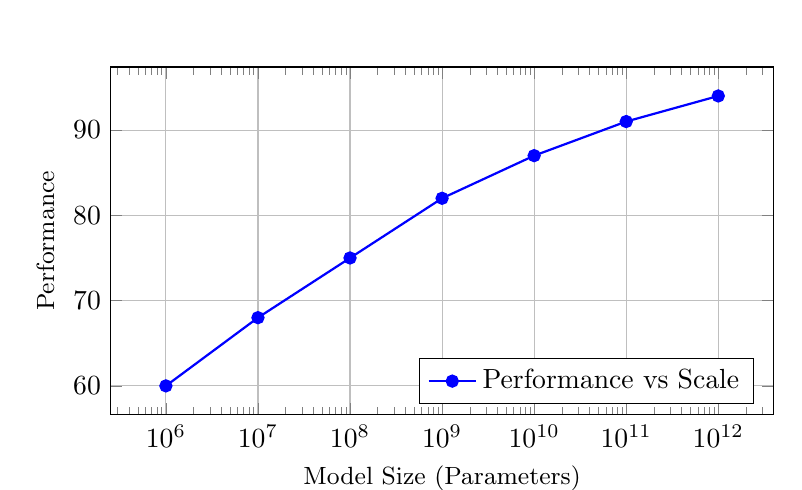
\begin{tikzpicture}
\begin{axis}[
    xlabel={Model Size (Parameters)},
    ylabel={Performance},
    xmode=log,
    log basis x=10,
    grid=major,
    width=10cm,
    height=6cm,
    legend pos=south east,
    xlabel style={font=\small},
    ylabel style={font=\small}
]
\addplot[
    color=blue,
    mark=*,
    thick
] coordinates {
    (1e6, 60)
    (1e7, 68)
    (1e8, 75)
    (1e9, 82)
    (1e10, 87)
    (1e11, 91)
    (1e12, 94)
};
\legend{Performance vs Scale}
\end{axis}
\end{tikzpicture}
\end{center}

\begin{center}
\textit{Illustration: As model size increases (log scale), performance improves following the scaling hypothesis.}
\end{center}

\section{The Attention Mechanism}

\subsection{Motivation: Context-Dependent Representations}

\begin{example}[Word Ambiguity]
Consider the following two sentences containing the word "bank":
\begin{itemize}
    \item \textit{I swam across the river to get to the other \textbf{bank}}
    \item \textit{I walked across the road to get cash from the \textbf{bank}}
\end{itemize}

To determine the exact interpretation of the word \textit{bank}, an artificial neural network should \textbf{rely more heavily on} (i.e., \textbf{attend to}) specific words from the rest of the sentence (\textbf{context}).

In the first sentence, "bank" should attend more to words like "river" and "swam" (indicating a riverbank). In the second sentence, "bank" should attend more to words like "cash" and "road" (indicating a financial institution).
\end{example}

\subsection{Attention vs. Standard Neural Networks}

\begin{tcolorbox}[colback=orange!10!white,colframe=orange!75!black,title=\textbf{Key Difference}]
\textbf{Standard neural networks}: When the network is trained, weights are \textbf{fixed}.

\textbf{Attention mechanism}: Uses \textbf{weighting factors} whose values \textbf{depend on the specific input data}.
\end{tcolorbox}

\begin{observation}
A Transformer can be seen as a \textbf{rich form of embedding} in which a given vector (e.g., representing a word) is mapped to a location that \textbf{depends on the other vectors} (i.e., words) of the sentence.

\textbf{Example}: The embedding of the word "bank" will be:
\begin{itemize}
    \item Close to "water" in the first sentence
    \item Close to "money" in the second sentence
\end{itemize}

This context-dependent representation is what makes Transformers so powerful for natural language understanding.
\end{observation}

\section{Transformer Processing: Mathematical Framework}

\subsection{Notation and Terminology}

\begin{definition}[Input Representation]
The input to a Transformer consists of:
\begin{itemize}
    \item \textbf{Set of vectors}: $\{x_n\}$ of dimensionality $D$ where $n = 1, \ldots, N$
    \item Each vector is called a \textbf{token}
\end{itemize}
\end{definition}

\subsubsection{What is a Token?}

A \textbf{token} is a fundamental unit of input data. Examples include:
\begin{itemize}
    \item A \textbf{word} in a sentence
    \item A \textbf{patch} in an image
    \item An \textbf{amino acid} in a protein sequence
    \item A \textbf{number or set of numbers} in a time series
\end{itemize}

\subsubsection{Features}

The elements $x_{ni}$ of a token are called \textbf{features}, where $i = 1, \ldots, D$.

\subsubsection{Data Matrix}

\begin{definition}[Data Matrix]
The \textbf{data matrix} (set of tokens) is denoted by $\mathbf{X}$ with dimension $N \times D$:
\begin{itemize}
    \item Each \textbf{row} is a token vector $\mathbf{x}_n^T$
    \item $N$ is the number of tokens
    \item $D$ is the number of features (dimensionality)
\end{itemize}

A \textbf{training set} contains many sets of tokens (i.e., many matrices).
\end{definition}

\begin{center}
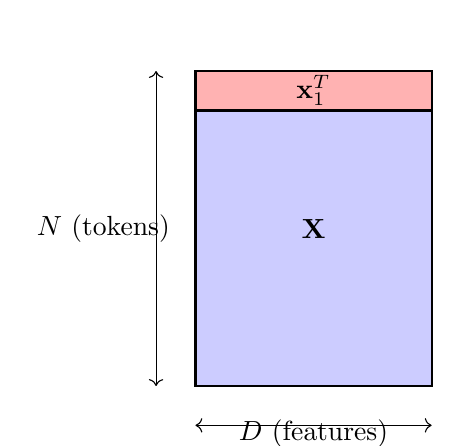
\begin{tikzpicture}
\draw[fill=blue!20, draw=black, thick] (0,0) rectangle (3,4);
\draw[fill=red!30, draw=black, thick] (0,3.5) rectangle (3,4);
\node at (1.5,3.75) {$\mathbf{x}_1^T$};
\node at (1.5,2) {$\mathbf{X}$};
\node[left] at (-0.2,2) {$N$ (tokens)};
\node[below] at (1.5,-0.3) {$D$ (features)};
\draw[<->] (-0.5,0) -- (-0.5,4);
\draw[<->] (0,-0.5) -- (3,-0.5);
\end{tikzpicture}
\end{center}

\subsection{Transformer Layer: The Main Building Block}

\begin{tcolorbox}[colback=blue!10!white,colframe=blue!75!black,title=\textbf{Transformer Layer}]
A \textbf{Transformer layer} is the fundamental building block of a Transformer that:
\begin{itemize}
    \item Takes a \textbf{data matrix} $\mathbf{X}$ as input
    \item Returns a \textbf{transformed matrix} $\tilde{\mathbf{X}}$ of the same dimension as output
\end{itemize}

\[
\tilde{\mathbf{X}} = \text{TransformerLayer}[\mathbf{X}]
\]
\end{tcolorbox}

\subsubsection{Key Properties}

\begin{enumerate}
    \item \textbf{Multiple layers}: Multiple Transformer layers can be applied in succession to learn \textbf{rich internal representations}
    
    \item \textbf{Learnable weights}: Each Transformer layer contains weights that can be learned by \textbf{gradient descent} using an appropriate \textbf{cost function}
    
    \item \textbf{Two-stage processing}: Each Transformer layer performs two stages:
    \begin{enumerate}
        \item \textbf{Stage 1 (Attention)}: Mixes features from different tokens across the \textbf{columns} of $\mathbf{X}$ (attention mechanism)
        \item \textbf{Stage 2 (Feed-forward)}: Transforms the values of each token acting on the \textbf{rows} of $\mathbf{X}$ independently
    \end{enumerate}
\end{enumerate}

\begin{center}
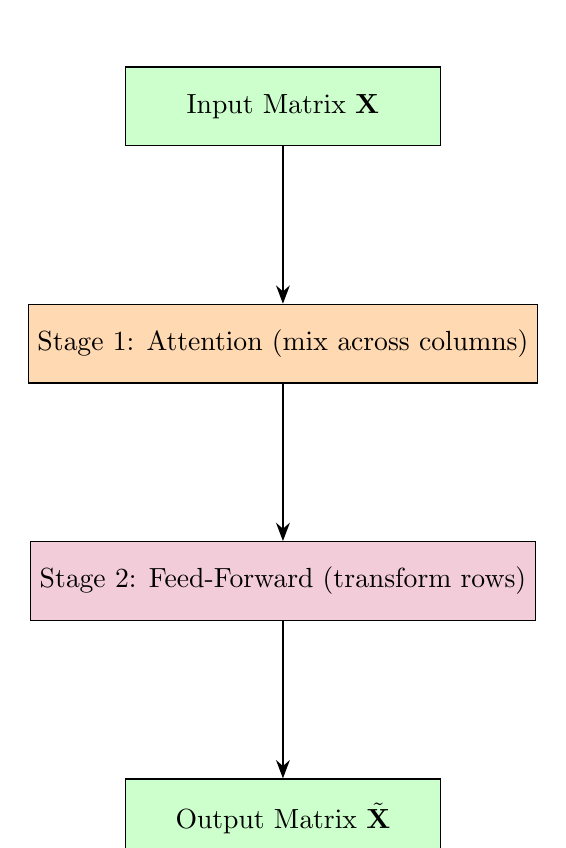
\begin{tikzpicture}[node distance=2cm]
\node[draw, rectangle, fill=green!20, minimum width=4cm, minimum height=1cm] (input) {Input Matrix $\mathbf{X}$};
\node[draw, rectangle, fill=orange!30, minimum width=4cm, minimum height=1cm, below=of input] (stage1) {Stage 1: Attention (mix across columns)};
\node[draw, rectangle, fill=purple!20, minimum width=4cm, minimum height=1cm, below=of stage1] (stage2) {Stage 2: Feed-Forward (transform rows)};
\node[draw, rectangle, fill=green!20, minimum width=4cm, minimum height=1cm, below=of stage2] (output) {Output Matrix $\tilde{\mathbf{X}}$};

\draw[-Stealth, thick] (input) -- (stage1);
\draw[-Stealth, thick] (stage1) -- (stage2);
\draw[-Stealth, thick] (stage2) -- (output);
\end{tikzpicture}
\end{center}

\section{Attention Coefficients}

\subsection{The Goal of Attention}

\begin{tcolorbox}[colback=cyan!10!white,colframe=cyan!75!black,title=\textbf{Attention Objective}]
Given a set of tokens in an embedding space: $\mathbf{x}_1, \ldots, \mathbf{x}_N$

\textbf{Goal}: Map them into another set $\mathbf{y}_1, \ldots, \mathbf{y}_N$ with richer semantic structure.

\textbf{Key principle}: The value of a generic output token $\mathbf{y}_n$ should \textbf{depend on all input tokens}.

\textbf{Attention}: The dependence should be \textbf{stronger} for inputs $\mathbf{x}_m$ particularly important for determining the new representation of $\mathbf{y}_n$.
\end{tcolorbox}

\subsection{Linear Combination Case}

In the simplest case, we can express the output as a \textbf{linear combination} of the input tokens:

\[
\mathbf{y}_n = \sum_{m=1}^{N} a_{nm} \mathbf{x}_m
\]

where:
\begin{itemize}
    \item $a_{nm}$ are called \textbf{attention weights}
    \item Constraint: $a_{nm} \geq 0$ and $\sum_{m=1}^{N} a_{nm} = 1$ (partition of unity to avoid compensation)
\end{itemize}

\begin{definition}[Attention Weights]
The coefficients $a_{nm}$ represent how much the $n$-th output token should "attend to" the $m$-th input token. They form a probability distribution over the input tokens for each output position.
\end{definition}

\textbf{Interpretation}:
\begin{itemize}
    \item If $a_{nm}$ is large, token $\mathbf{x}_m$ has a strong influence on $\mathbf{y}_n$
    \item If $a_{nm}$ is small, token $\mathbf{x}_m$ has little influence on $\mathbf{y}_n$
    \item The sum constraint ensures that the total attention is normalized
\end{itemize}

\section{Self-Attention Mechanism}

\subsection{How to Compute Attention Coefficients}

\subsubsection{Example: Movie Selection (Hard Attention)}

To understand how attention coefficients work, consider a simplified example of movie selection based on user preferences.

\begin{example}[Movie Recommendation with Hard Attention]
Given:
\begin{itemize}
    \item \textbf{Preference (query)}: A user's preference vector representing their interests
    \item \textbf{Movies database}: A collection of movies, each with:
    \begin{itemize}
        \item \textbf{Keys}: Feature vectors describing movie properties
        \item \textbf{Values}: The actual movie content/representation
    \end{itemize}
\end{itemize}

The system computes a \textbf{similarity score} $Q^TK$ between the user's query and each movie's key. In \textbf{hard attention}, only the movie with the highest similarity score is selected.
\end{example}

\subsection{Self-Attention in Transformers}

In Transformers, the attention mechanism is more sophisticated than the hard attention example above. Here's how it works:

\begin{tcolorbox}[colback=purple!10!white,colframe=purple!75!black,title=\textbf{Self-Attention: Key Concepts}]
\begin{itemize}
    \item Each input token $\mathbf{x}_n$ serves \textbf{both} as a \textbf{key} and a \textbf{value} (i.e., the token itself summarizes its features)
    
    \item The token $\mathbf{x}_m$ is used as a \textbf{query} for the output $\mathbf{y}_m$ (then $\mathbf{x}_m$ is compared to all the key tokens)
    
    \item The dot product $\mathbf{x}_n^T \mathbf{x}_m$ is used to compute the \textbf{query-key similarity}, which determines how much the token represented by $\mathbf{x}_n$ should \textbf{attend to} the token represented by $\mathbf{x}_m$ (i.e., how $\mathbf{x}_n$ is important to generate $\mathbf{y}_m$)
\end{itemize}
\end{tcolorbox}

\subsubsection{Computing Attention Weights with Softmax}

Constraints are imposed using the \textbf{softmax function}:

\[
a_{nm} = \frac{\exp(\mathbf{x}_n^T \mathbf{x}_m)}{\sum_{m'=1}^{N} \exp(\mathbf{x}_n^T \mathbf{x}_{m'})}
\]

This formula ensures:
\begin{itemize}
    \item All attention weights are positive: $a_{nm} > 0$
    \item They sum to one: $\sum_{m=1}^{N} a_{nm} = 1$
    \item Higher dot products yield higher attention weights (exponential scaling)
\end{itemize}

\subsection{Summary: Self-Attention Transformation}

\begin{tcolorbox}[colback=red!10!white,colframe=red!75!black,title=\textbf{Self-Attention Formula}]
Each \textbf{input vector} $\mathbf{x}_n$ is transformed to a corresponding \textbf{output vector} $\mathbf{y}_n$ by taking a \textbf{linear combination} of input vectors:

\[
\mathbf{y}_n = \sum_{m=1}^{N} a_{nm} \mathbf{x}_m
\]

where the weight $a_{nm}$ applied to vector $\mathbf{x}_m$ is computed by the softmax of the dot-product between the \textbf{query} $\mathbf{x}_n$ and the \textbf{key} $\mathbf{x}_m$.
\end{tcolorbox}

\subsubsection{Matrix Notation}

In matrix form, the self-attention operation can be written as:

\[
\mathbf{Y} = \text{Softmax}[\mathbf{X}\mathbf{X}^T]\mathbf{X}
\]

where:
\begin{itemize}
    \item $\mathbf{X}$ is the $N \times D$ input matrix (N tokens, D features)
    \item $\mathbf{X}^T$ is the $D \times N$ transpose
    \item $\mathbf{X}\mathbf{X}^T$ is an $N \times N$ similarity matrix
    \item Softmax is applied row-wise to normalize each row
    \item $\mathbf{Y}$ is the $N \times D$ output matrix
\end{itemize}

\textbf{Interpretation of $\mathbf{X}\mathbf{X}^T$}:
\begin{itemize}
    \item This is an $N \times N$ matrix where element $(n,m)$ contains $\mathbf{x}_n^T \mathbf{x}_m$
    \item Each row represents how similar token $n$ is to all other tokens
    \item After softmax, each row becomes the attention weights for that token
\end{itemize}

\section{Learnable Parameters in Self-Attention}

\subsection{The Problem with Simple Self-Attention}

\begin{observation}
The basic self-attention transformation $\mathbf{Y} = \text{Softmax}[\mathbf{X}\mathbf{X}^T]\mathbf{X}$ has \textbf{no learnable parameters}.

Additionally, each feature value within a token vector $\mathbf{x}_n$ plays an \textbf{equal role} in determining the attention coefficients. This limits the expressiveness of the model.
\end{observation}

\subsection{Solution: Query, Key, and Value Transformations}

\begin{tcolorbox}[colback=green!10!white,colframe=green!75!black,title=\textbf{Modified Feature Vectors}]
Define \textbf{modified feature vectors} as linear transformations of the original vectors:

\begin{align*}
\mathbf{Q} &= \mathbf{X}\mathbf{W}^{(q)} && \text{(Queries)} \\
\mathbf{K} &= \mathbf{X}\mathbf{W}^{(k)} && \text{(Keys)} \\
\mathbf{V} &= \mathbf{X}\mathbf{W}^{(v)} && \text{(Values)}
\end{align*}

where $\mathbf{W}^{(q)}$, $\mathbf{W}^{(k)}$, and $\mathbf{W}^{(v)}$ are \textbf{learnable parameter matrices}.
\end{tcolorbox}

\subsubsection{Dimensions}

The weight matrices have the following dimensions:
\begin{itemize}
    \item $\mathbf{W}^{(q)}$: $D \times D_q$ (not necessarily $D_q = D$)
    \item $\mathbf{W}^{(k)}$: $D \times D_k$
    \item $\mathbf{W}^{(v)}$: $D \times D_v$
\end{itemize}

Usually, $D_k = D_v = D$, so:
\begin{itemize}
    \item Dimension of output = dimension of input
    \item \textbf{Multiple Transformer layers can be stacked} sequentially
\end{itemize}

\subsubsection{Resulting Matrices}

After transformation:
\begin{itemize}
    \item $\mathbf{Q}$: $N \times D_q$ matrix of query vectors
    \item $\mathbf{K}$: $N \times D_k$ matrix of key vectors  
    \item $\mathbf{V}$: $N \times D_v$ matrix of value vectors
\end{itemize}

\subsection{Modified Self-Attention Formula}

With the learnable transformations, the self-attention mechanism becomes:

\[
\mathbf{Y} = \text{Softmax}\left[\mathbf{Q}\mathbf{K}^T\right]\mathbf{V}
\]

or equivalently:

\[
\mathbf{Y} = \text{Softmax}\left[\mathbf{X}\mathbf{W}^{(q)}\left(\mathbf{X}\mathbf{W}^{(k)}\right)^T\right]\mathbf{X}\mathbf{W}^{(v)}
\]

\textbf{Key benefits}:
\begin{itemize}
    \item The model can \textbf{learn} which features are important for queries, keys, and values
    \item Different features can play different roles in computing attention
    \item The weight matrices $\mathbf{W}^{(q)}$, $\mathbf{W}^{(k)}$, $\mathbf{W}^{(v)}$ are trained via gradient descent
\end{itemize}

\subsection{General Formula and Dimensions}

\begin{tcolorbox}[colback=blue!10!white,colframe=blue!75!black,title=\textbf{General Self-Attention Formula}]
The general formula for computing the self-attention transformation is:

\[
\mathbf{Y} = \text{Softmax}[\mathbf{Q}\mathbf{K}^T]\mathbf{V}
\]

where:
\begin{itemize}
    \item $\mathbf{Q}\mathbf{K}^T$ has dimension $N \times N$ (attention weight matrix)
    \item $\mathbf{Y}$ has dimension $N \times D_v$ (output matrix)
\end{itemize}
\end{tcolorbox}

\subsubsection{Dimensional Analysis}

Let's trace through the dimensions step by step:

\begin{enumerate}
    \item \textbf{Input}: $\mathbf{X}$ has dimension $N \times D$
    
    \item \textbf{Query transformation}: 
    \[
    \mathbf{Q} = \mathbf{X}\mathbf{W}^{(q)}
    \]
    \begin{itemize}
        \item $\mathbf{X}$: $N \times D$
        \item $\mathbf{W}^{(q)}$: $D \times D$
        \item $\mathbf{Q}$: $N \times D$
    \end{itemize}
    
    \item \textbf{Key transformation}:
    \[
    \mathbf{K} = \mathbf{X}\mathbf{W}^{(k)}
    \]
    \begin{itemize}
        \item $\mathbf{X}$: $N \times D$
        \item $\mathbf{W}^{(k)}$: $D \times D$
        \item $\mathbf{K}$: $N \times D$
    \end{itemize}
    
    \item \textbf{Attention scores}:
    \[
    \mathbf{Q}\mathbf{K}^T
    \]
    \begin{itemize}
        \item $\mathbf{Q}$: $N \times D$
        \item $\mathbf{K}^T$: $D \times N$
        \item $\mathbf{Q}\mathbf{K}^T$: $N \times N$
    \end{itemize}
    
    \item \textbf{Value transformation}:
    \[
    \mathbf{V} = \mathbf{X}\mathbf{W}^{(v)}
    \]
    \begin{itemize}
        \item $\mathbf{X}$: $N \times D$
        \item $\mathbf{W}^{(v)}$: $D \times D_v$
        \item $\mathbf{V}$: $N \times D_v$
    \end{itemize}
    
    \item \textbf{Final output}:
    \[
    \mathbf{Y} = \text{Softmax}[\mathbf{Q}\mathbf{K}^T]\mathbf{V}
    \]
    \begin{itemize}
        \item $\text{Softmax}[\mathbf{Q}\mathbf{K}^T]$: $N \times N$
        \item $\mathbf{V}$: $N \times D_v$
        \item $\mathbf{Y}$: $N \times D_v$
    \end{itemize}
\end{enumerate}

\begin{center}
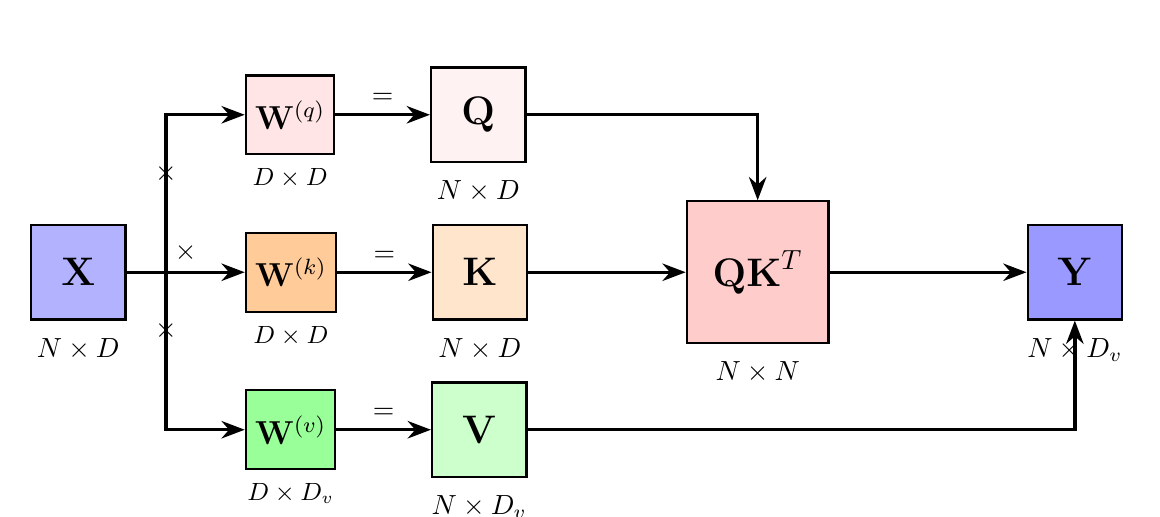
\begin{tikzpicture}[scale=1.0,
    box/.style={rectangle, draw=black, thick, minimum width=1.2cm, minimum height=1.2cm},
    smallbox/.style={rectangle, draw=black, thick, minimum width=1cm, minimum height=1cm}
]

% X matrix (left)
\node[box, fill=blue!30] (X) at (0,0) {\Large $\mathbf{X}$};
\node[below=0.1cm of X] {$N \times D$};

% W^(q) and Q (top branch)
\node[smallbox, fill=pink!40, right=1.5cm of X, yshift=2cm] (Wq) {\large $\mathbf{W}^{(q)}$};
\node[below=0.05cm of Wq, font=\small] {$D \times D$};

\node[box, fill=pink!20, right=1.2cm of Wq] (Q) {\Large $\mathbf{Q}$};
\node[below=0.1cm of Q] {$N \times D$};

% W^(k) and K (middle branch)
\node[smallbox, fill=orange!40, right=1.5cm of X] (Wk) {\large $\mathbf{W}^{(k)}$};
\node[below=0.05cm of Wk, font=\small] {$D \times D$};

\node[box, fill=orange!20, right=1.2cm of Wk] (K) {\Large $\mathbf{K}$};
\node[below=0.1cm of K] {$N \times D$};

% W^(v) and V (bottom branch)
\node[smallbox, fill=green!40, right=1.5cm of X, yshift=-2cm] (Wv) {\large $\mathbf{W}^{(v)}$};
\node[below=0.05cm of Wv, font=\small] {$D \times D_v$};

\node[box, fill=green!20, right=1.2cm of Wv] (V) {\Large $\mathbf{V}$};
\node[below=0.1cm of V] {$N \times D_v$};

% QK^T (attention scores)
\node[box, fill=red!20, minimum width=1.8cm, minimum height=1.8cm, right=2cm of K] (QKT) {\Large $\mathbf{QK}^T$};
\node[below=0.1cm of QKT] {$N \times N$};

% Y (output)
\node[box, fill=blue!40, right=2.5cm of QKT] (Y) {\Large $\mathbf{Y}$};
\node[below=0.1cm of Y] {$N \times D_v$};

% Arrows from X
\draw[-Stealth, very thick] (X.east) -- ++(0.5,0) |- (Wq.west) node[pos=0.25, above] {$\times$};
\draw[-Stealth, very thick] (X.east) -- (Wk.west) node[midway, above] {$\times$};
\draw[-Stealth, very thick] (X.east) -- ++(0.5,0) |- (Wv.west) node[pos=0.25, above] {$\times$};

% Arrows from W to Q, K, V
\draw[-Stealth, very thick] (Wq.east) -- (Q.west) node[midway, above] {$=$};
\draw[-Stealth, very thick] (Wk.east) -- (K.west) node[midway, above] {$=$};
\draw[-Stealth, very thick] (Wv.east) -- (V.west) node[midway, above] {$=$};

% Arrows from Q and K to QK^T
\draw[-Stealth, very thick] (Q.east) -| (QKT.north);
\draw[-Stealth, very thick] (K.east) -- (QKT.west);

% Arrows from QK^T and V to Y
\draw[-Stealth, very thick] (QKT.east) -- (Y.west);
\draw[-Stealth, very thick] (V.east) -| (Y.south);

\end{tikzpicture}
\end{center}

\subsection{Key Distinction: Data-Dependent Attention}

\begin{tcolorbox}[colback=red!10!white,colframe=red!75!black,title=\textbf{Important Notice}]
\textbf{Standard neural networks} multiply activations by \textbf{fixed weights}.

\textbf{Transformers} multiply activations by \textbf{data-dependent attention coefficients}.

This is a fundamental difference that gives Transformers their power and flexibility.
\end{tcolorbox}

\subsubsection{Example: Input-Specific Attention}

\begin{example}[Selective Attention]
Consider two different input vectors $\mathbf{x}'$ and $\mathbf{x}''$:

\begin{itemize}
    \item An attention coefficient could be \textbf{close to zero} for input vector $\mathbf{x}'$
    \begin{itemize}
        \item This means the incoming signal is \textbf{ignored} in the signal path
    \end{itemize}
    
    \item The same attention coefficient could be \textbf{very large} for another input vector $\mathbf{x}''$
    \begin{itemize}
        \item This means the incoming signal is \textbf{strongly considered}
    \end{itemize}
\end{itemize}

\textbf{Key insight}: By contrast, if a standard neural network learns to ignore an input, it does so \textbf{for all input vectors}. The network cannot selectively attend based on context.
\end{example}

\begin{observation}
This data-dependent weighting allows Transformers to:
\begin{itemize}
    \item \textbf{Dynamically route information} based on input content
    \item \textbf{Context-sensitive processing}: The same token can be processed differently depending on surrounding tokens
    \item \textbf{Flexible feature selection}: Different features become important for different inputs
    \item \textbf{Adaptive computation}: The network's effective structure changes with each input
\end{itemize}

This is why Transformers excel at tasks requiring understanding of context and relationships between elements, such as natural language processing and sequence modeling.
\end{observation}

\section{Multi-Head Attention}

\subsection{Limitation of Single Attention Head}

\begin{observation}
While self-attention provides a powerful mechanism for capturing relationships between tokens, a single attention head may not capture all types of relationships effectively. Different aspects of the input may require different attention patterns.
\end{observation}

\subsection{The Multi-Head Solution}

\begin{tcolorbox}[colback=green!10!white,colframe=green!75!black,title=\textbf{Multi-Head Attention}]
\textbf{Multi-head attention} allows the model to attend to information from different representation subspaces simultaneously. Instead of computing a single attention function, we compute $h$ parallel attention functions (heads).
\end{tcolorbox}

\subsubsection{Mathematical Formulation}

For each head $i = 1, \ldots, h$:

\begin{align*}
\mathbf{Q}^{(i)} &= \mathbf{X}\mathbf{W}^{(q,i)} \\
\mathbf{K}^{(i)} &= \mathbf{X}\mathbf{W}^{(k,i)} \\
\mathbf{V}^{(i)} &= \mathbf{X}\mathbf{W}^{(v,i)}
\end{align*}

Each head computes its own attention:

\[
\mathbf{Y}^{(i)} = \text{Softmax}\left[\frac{\mathbf{Q}^{(i)}\mathbf{K}^{(i)T}}{\sqrt{d_k}}\right]\mathbf{V}^{(i)}
\]

The outputs of all heads are concatenated and linearly transformed:

\[
\mathbf{Y} = \text{Concat}(\mathbf{Y}^{(1)}, \ldots, \mathbf{Y}^{(h)})\mathbf{W}^{(o)}
\]

\subsubsection{Why Multi-Head?}

\begin{itemize}
    \item \textbf{Different perspectives}: Each head can learn to focus on different types of relationships
    \item \textbf{Parallel processing}: All heads process the input simultaneously
    \item \textbf{Richer representations}: Multiple heads capture more complex patterns
    \item \textbf{Stability}: The $\sqrt{d_k}$ scaling prevents gradients from becoming too small
\end{itemize}

\begin{example}[Multi-Head Attention in Action]
Consider the sentence: "The bank by the river is beautiful"

\begin{itemize}
    \item \textbf{Head 1} might focus on syntactic relationships (subject-verb)
    \item \textbf{Head 2} might focus on semantic relationships (bank-river)
    \item \textbf{Head 3} might focus on positional relationships
    \item \textbf{Head 4} might focus on morphological patterns
\end{itemize}

Each head learns different attention patterns, providing a comprehensive understanding of the input.
\end{example}

\section{Positional Encoding}

\subsection{The Need for Position Information}

\begin{tcolorbox}[colback=orange!10!white,colframe=orange!75!black,title=\textbf{Problem: Permutation Invariance}]
Transformers are inherently \textbf{permutation invariant}—they treat input tokens as an unordered set. However, in sequences like text, \textbf{position matters}:

\begin{itemize}
    \item "The cat sat on the mat" $\neq$ "The mat sat on the cat"
    \item "I love you" $\neq$ "You love I"
\end{itemize}
\end{tcolorbox}

\subsection{Solution: Positional Encoding}

\begin{definition}[Positional Encoding]
\textbf{Positional encoding} adds position-specific information to token embeddings so that the transformer can distinguish between tokens based on their position in the sequence.
\end{definition}

\subsubsection{Sinusoidal Positional Encoding}

The original Transformer paper uses sinusoidal functions:

\[
\text{PE}(pos, 2i) = \sin\left(\frac{pos}{10000^{2i/d_{model}}}\right)
\]
\[
\text{PE}(pos, 2i+1) = \cos\left(\frac{pos}{10000^{2i/d_{model}}}\right)
\]

where:
\begin{itemize}
    \item $pos$ is the position in the sequence
    \item $i$ is the dimension index
    \item $d_{model}$ is the model dimension
\end{itemize}

\subsubsection{Learned Positional Embeddings}

Modern approaches often use learned embeddings:

\[
\mathbf{x}_n = \mathbf{x}_n + \mathbf{p}_n
\]

where $\mathbf{p}_n$ is a learned vector specific to position $n$.

\subsection{Properties of Good Positional Encoding}

\begin{observation}
Effective positional encoding should satisfy:
\begin{itemize}
    \item \textbf{Unique for each position}: Different positions should have different encodings
    \item \textbf{Consistent for similar distances}: Positions $i$ and $j$ should have similar encodings if $|i-j|$ is small
    \item \textbf{Generalizable}: Should work for sequences longer than seen during training
    \item \textbf{Additive}: Should not interfere with the semantic meaning of tokens
\end{itemize}
\end{observation}

\section{The Complete Transformer Architecture}

\subsection{Encoder-Decoder Structure}

\begin{tcolorbox}[colback=blue!10!white,colframe=blue!75!black,title=\textbf{Transformer Architecture}]
The Transformer consists of an \textbf{encoder} and a \textbf{decoder}, both composed of stacked layers:

\begin{itemize}
    \item \textbf{Encoder}: Processes the input sequence and creates contextual representations
    \item \textbf{Decoder}: Generates the output sequence using encoder outputs and previously generated tokens
\end{itemize}
\end{tcolorbox}

\subsubsection{Encoder Stack}

Each encoder layer contains:
\begin{enumerate}
    \item \textbf{Multi-head attention}: Self-attention over input tokens
    \item \textbf{Feed-forward network}: Point-wise transformations
    \item \textbf{Residual connections} and \textbf{layer normalization}
\end{enumerate}

\subsubsection{Decoder Stack}

Each decoder layer contains:
\begin{enumerate}
    \item \textbf{Masked multi-head attention}: Self-attention over target tokens (masked to prevent peeking)
    \item \textbf{Multi-head attention}: Attention over encoder outputs
    \item \textbf{Feed-forward network}
    \item \textbf{Residual connections} and \textbf{layer normalization}
\end{enumerate}

\subsection{Layer Normalization and Residual Connections}

\begin{definition}[Residual Connection]
A \textbf{residual connection} adds the input of a layer to its output:

\[
\mathbf{y} = \mathbf{x} + \text{Layer}(\mathbf{x})
\]
\end{definition}

\begin{definition}[Layer Normalization]
\textbf{Layer normalization} normalizes the features within each sample:

\[
\text{LayerNorm}(\mathbf{x}) = \gamma \cdot \frac{\mathbf{x} - \mu}{\sqrt{\sigma^2 + \epsilon}} + \beta
\]
\end{definition}

\section{Transformer Layers}

\subsection{Multi-Head Attention Algorithm}

\begin{observation}
Multi-head attention allows the model to simultaneously attend to information from different representation subspaces. Each head learns independent query, key, and value transformations, enabling diverse attention patterns.
\end{observation}

\begin{tcolorbox}[colback=red!10!white,colframe=red!75!black,title=\textbf{Algorithm 12.2: Multi-head attention}]
\textbf{Input:} Set of tokens $\mathbf{X} \in \mathbb{R}^{N \times D}$: $\{x_1, \ldots, x_N\}$

Query weight matrices $\{\mathbf{W}_1^{(q)}, \ldots, \mathbf{W}_H^{(q)}\} \in \mathbb{R}^{D \times D}$ (one per head)

Key weight matrices $\{\mathbf{W}_1^{(k)}, \ldots, \mathbf{W}_H^{(k)}\} \in \mathbb{R}^{D \times D}$ (one per head)

Value weight matrices $\{\mathbf{W}_1^{(v)}, \ldots, \mathbf{W}_H^{(v)}\} \in \mathbb{R}^{D \times D_v}$ (one per head)

Output weight matrix $\mathbf{W}^{(o)} \in \mathbb{R}^{HD_v \times D}$ (projects concatenated heads back to original dimension)

\textbf{Output:} $\mathbf{Y} \in \mathbb{R}^{N \times D}$: $\{y_1, \ldots, x_N\}$

\vspace{0.3cm}

\textcolor{blue}{// compute self-attention for each head (Algorithm 12.1)}

\textbf{for} $h = 1, \ldots, H$ \textbf{do}

\quad $\mathbf{Q}_h = \mathbf{X}\mathbf{W}_h^{(q)}$, $\mathbf{K}_h = \mathbf{X}\mathbf{W}_h^{(k)}$, $\mathbf{V}_h = \mathbf{X}\mathbf{W}_h^{(v)}$ \textcolor{blue}{// project inputs for this head}

\quad $\mathbf{H}_h = \text{Attention}(\mathbf{Q}_h, \mathbf{K}_h, \mathbf{V}_h)$ \textcolor{blue}{// $\mathbf{H}_h \in \mathbb{R}^{N \times D_v}$}

\textbf{end for}

$\mathbf{H} = \text{Concat}[\mathbf{H}_1, \ldots, \mathbf{H}_N]$ \textcolor{blue}{// concatenate all head outputs: $\mathbf{H} \in \mathbb{R}^{N \times HD_v}$}

\textbf{return} $\mathbf{Y}(\mathbf{X}) = \mathbf{H}\mathbf{W}^{(o)}$ \textcolor{blue}{// project back to original dimension}
\end{tcolorbox}

\subsubsection{Key Insights}

\begin{itemize}
    \item Each head operates independently with its own learnable transformations, allowing different heads to capture different types of relationships
    \item The concatenation of all heads produces a richer representation than a single attention head
    \item The output projection $\mathbf{W}^{(o)}$ combines information from all heads and maps back to the original dimension $D$
\end{itemize}

\subsection{Transformer Layer Structure}

\begin{definition}[Residual Connection]
A residual connection (or skip connection) adds the input directly to the output of a layer: $\text{output} = \text{Layer}(\text{input}) + \text{input}$. This enables gradients to flow directly through the network during backpropagation.
\end{definition}

\begin{itemize}
    \item \textbf{Multi-head self-attention is the core of transformer layers} - it enables the model to attend to different parts of the input simultaneously
    
    \item \textbf{To improve training efficiency we introduce residual connections} that bypass the multi-head structure - this helps with gradient flow and allows information to propagate directly through layers
    
    \item \textbf{Then, layer normalization} (Ba, Kiros, and Hinton, 2016) is performed, which also improves training efficiency - it stabilizes training by normalizing the distribution of layer inputs
    
    \item \textbf{Resulting transformation:}
    \[
    \mathbf{Z} = \text{LayerNorm}[\mathbf{Y}(\mathbf{X}) + \mathbf{X}]
    \]
    
    This combines the attention output with the original input and normalizes the result.
\end{itemize}

\subsection{Nonlinearity and Feed-Forward Network}

\begin{observation}
The attention mechanism, while powerful, has a fundamental limitation: it produces outputs that are linear combinations of the input value vectors. This constrains the expressiveness of the layer.
\end{observation}

\begin{itemize}
    \item \textbf{Problem:} the attention mechanism creates linear combinations of the value vectors, which are linearly combined to produce output vectors. So, \textcolor{red}{\textbf{outputs of attention layers are constrained to be linear combinations of the inputs}}.
    
    \item \textcolor{red}{\textbf{Nonlinearity enters only in the attention weights (softmax function) but the output vectors are constrained to lie in the subspace spanned by the input vectors, which limits the expressiveness of the attention layer}}
    
    \item \textbf{Solution:} We can enhance the flexibility by \textbf{post-processing the output of each layer using a standard nonlinear neural network with $D$ inputs and $D$ outputs (MLP[·])}. E.g., two-layer fully connected with ReLU hidden units
    
    \begin{itemize}
        \item This feed-forward network introduces nonlinearity that allows the model to learn more complex transformations
        \item The MLP typically has a hidden layer with more units than $D$ (e.g., $4D$) to increase model capacity
    \end{itemize}
    
    \item \textbf{Notice:} the same shared network is applied to each of the output vectors (i.e., tokens, rows of $\mathbf{Z}$) - this is called a position-wise feed-forward network
    
    \item \textbf{Residual connections and layer normalization} are applied also to this stage, to improve training efficiency and enable deeper networks
\end{itemize}

\subsection{Complete Transformer Layer}

\begin{tcolorbox}[colback=blue!10!white,colframe=blue!75!black,title=\textbf{Final output of the transformer layer}]
\[
\tilde{\mathbf{X}} = \text{LayerNorm}[\text{MLP}[\mathbf{Z}] + \mathbf{Z}]
\]
\end{tcolorbox}

\begin{center}
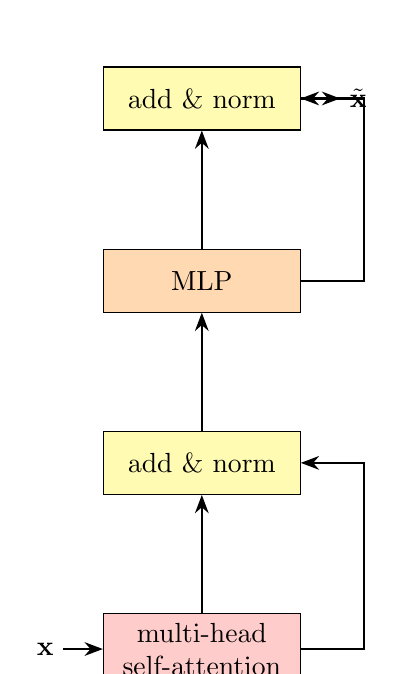
\begin{tikzpicture}[node distance=1.5cm]
\node[draw, rectangle, fill=red!20, minimum width=2.5cm, minimum height=0.8cm, align=center] (mha) {multi-head \\ self-attention};
\node[draw, rectangle, fill=yellow!30, minimum width=2.5cm, minimum height=0.8cm, above=of mha] (norm1) {add \& norm};
\node[draw, rectangle, fill=orange!30, minimum width=2.5cm, minimum height=0.8cm, above=of norm1] (mlp) {MLP};
\node[draw, rectangle, fill=yellow!30, minimum width=2.5cm, minimum height=0.8cm, above=of mlp] (norm2) {add \& norm};

\node[left=0.5cm of mha] (x) {$\mathbf{x}$};
\node[right=0.5cm of norm2] (xbar) {$\tilde{\mathbf{x}}$};

\draw[-Stealth, thick] (x) -- (mha);
\draw[-Stealth, thick] (mha) -- (norm1);
\draw[-Stealth, thick] (norm1) -- (mlp);
\draw[-Stealth, thick] (mlp) -- (norm2);
\draw[-Stealth, thick] (norm2) -- (xbar);

\draw[-Stealth, thick] (mha.east) -- ++(0.8,0) |- (norm1.east);
\draw[-Stealth, thick] (mlp.east) -- ++(0.8,0) |- (norm2.east);
\end{tikzpicture}
\end{center}

\begin{center}
\textit{Courtesy of Bishop et al., 2024}
\end{center}

\subsection{Transformer Layer Algorithm}

\begin{observation}
A complete transformer layer combines multi-head attention with a feed-forward network, connected via residual connections and layer normalization. This design enables the model to learn both attention-based relationships and complex nonlinear transformations.
\end{observation}

\begin{tcolorbox}[colback=red!10!white,colframe=red!75!black,title=\textbf{Algorithm 12.3: Transformer layer}]
\textbf{Input:} Set of tokens $\mathbf{X} \in \mathbb{R}^{N \times D}$: $\{x_1, \ldots, x_N\}$

Multi-head self-attention layer parameters (from Algorithm 12.2)

Feed-forward network parameters (typically a 2-layer MLP with ReLU activation)

\textbf{Output:} $\tilde{\mathbf{X}} \in \mathbb{R}^{N \times D}$: $\{\tilde{x}_1, \ldots, \tilde{x}_N\}$ (same dimension as input)

\vspace{0.3cm}

$\mathbf{Z} = \text{LayerNorm}[\mathbf{Y}(\mathbf{X}) + \mathbf{X}]$ \textcolor{blue}{// Apply attention, add residual, normalize}

$\tilde{\mathbf{X}} = \text{LayerNorm}[\text{MLP}[\mathbf{Z}] + \mathbf{Z}]$ \textcolor{blue}{// Apply MLP, add residual, normalize}

\textbf{return} $\tilde{\mathbf{X}}$
\end{tcolorbox}

\subsubsection{Design Rationale}

\begin{itemize}
    \item \textbf{Residual connections:} Enable gradients to flow directly through the network, facilitating training of deep models
    \item \textbf{Layer normalization:} Stabilizes training by normalizing activations, reducing internal covariate shift
    \item \textbf{Post-norm architecture:} Normalizing after each sub-layer (attention and MLP) has been shown to improve training stability
    \item \textbf{Dimension preservation:} The output has the same dimension as the input, allowing layers to be stacked sequentially
\end{itemize}

\section{Computational Complexity of the Attention Layer}

\subsection{Attention Layer Complexity}

\begin{tcolorbox}[colback=yellow!10!white,colframe=yellow!60!black,title=\textbf{Notation}]
$N$ vectors (tokens), $D$ dimension
\end{tcolorbox}

\begin{itemize}
    \item \textbf{Attention layer}
    \begin{itemize}
        \item Matrices $\mathbf{W}^{(q)}$, $\mathbf{W}^{(k)}$, and $\mathbf{W}^{(v)}$ have $\mathcal{O}(D^2)$ parameters and are shared across input tokens
        \item Matrices $\mathbf{Q}$, $\mathbf{K}$, and $\mathbf{V}$ have $\mathcal{O}(ND)$ parameters
        \item \textbf{Total computational cost for attention} $\big(\text{Softmax}[\frac{\mathbf{Q}\mathbf{K}^T}{\sqrt{D_k}}] \, \mathbf{V}\big)$: $\mathcal{O}(N^2 D)$
    \end{itemize}
    \item \textbf{MLP (after attention)}
    \begin{itemize}
        \item $D$ inputs, $D$ outputs
        \item Computational cost of a forward pass (for \emph{1 token}): $\mathcal{O}(D^2)$
        \item \textbf{Total computational cost (for $N$ tokens)}: $\mathcal{O}(ND^2)$
    \end{itemize}
    \item Depending on $N$ and $D$ the transformer layer or the MLP layer may dominate the computational cost
\end{itemize}

\subsection{Comparison with Fully Connected Network}

\begin{tcolorbox}[colback=yellow!10!white,colframe=yellow!60!black,title=\textbf{Notation}]
$N$ vectors (tokens), $D$ dimension
\end{tcolorbox}

\begin{itemize}
    \item \textbf{Standard fully connected network}
    \begin{itemize}
        \item Input/output size: $ND$
        \item Number of independent parameters: $\mathcal{O}(N^2 D^2)$
        \item Computational cost of a forward pass: $\mathcal{O}(N^2 D^2)$
    \end{itemize}
    \item \textbf{Conclusion:} Compared to a standard fully connected network (complexity $\mathcal{O}(N^2 D^2)$) a transformer layer (complexity $\max(\mathcal{O}(ND^2), \, \mathcal{O}(N^2 D))$) is computationally more efficient
\end{itemize}



\section{Tokenization: One-Hot Representation}

\subsection{How to Compute Token Vectors for a Given Text?}

\begin{itemize}
    \item Example: \textit{"Hello, I'm a language model,"}
\end{itemize}

\subsection{One-Hot Representation}

\begin{itemize}
    \item Fixed dictionary of words
    \item Vectors of length equal to the dictionary size
    \item $k$-th word has 1 in position $k$, 0 elsewhere
    \item \textbf{Problem:} Huge dimensionality of the dictionary and the tokens
\end{itemize}



\section{Tokenization: Byte Pair Encoding}

\subsection{Motivation}

\begin{tcolorbox}[colback=yellow!5!white,colframe=yellow!75!black,title=\textbf{One-Hot Encoding Issues}]
The \textbf{one-hot encoding} approach has a large dictionary size, which can become inefficient. To address this issue, we could use a dictionary of characters instead of words. However, this approach would discard the \textbf{semantically important word structure} of the language.
\end{tcolorbox}

\subsection{Byte Pair Encoding (BPE)}

\begin{tcolorbox}[colback=green!5!white,colframe=green!75!black,title=\textbf{Definition: Byte Pair Encoding}]
Byte Pair Encoding (BPE) provides an intermediate solution, acting as a compromise between character-level and word-level tokenization. BPE is a compression method adapted for tokenization. The process works as follows:
\begin{enumerate}
    \item Start with individual characters.
    \item Search a body of text for the most frequently occurring adjacent pairs of tokens.
    \item Replace the adjacent pair with a new token and add the token to the dictionary (note: new tokens cannot contain spaces).
    \item Repeat the process until a predefined number of tokens is reached.
\end{enumerate}
\end{tcolorbox}

\begin{figure}[h!]
\centering
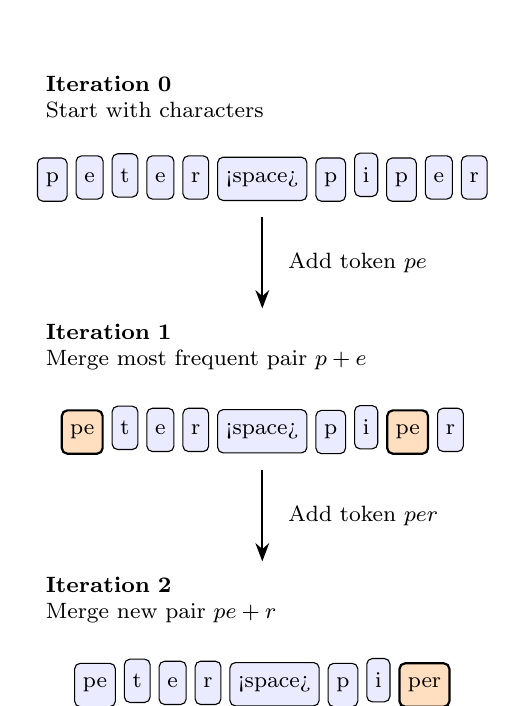
\begin{tikzpicture}[
    font=\footnotesize,
    token/.style={rectangle, draw, rounded corners=2pt, minimum height=0.55cm, inner xsep=3pt, fill=blue!8},
    merged/.style={token, fill=orange!25, thick},
    stage/.style={align=left, text width=5.5cm},
    arrow/.style={-Stealth, thick, shorten >=2pt, shorten <=2pt}
]
\node[stage] (iter0) {\textbf{Iteration 0}\\Start with characters};
\matrix (m0) [matrix of nodes, nodes=token, row sep=0mm, column sep=1mm, below=2mm of iter0] {
p & e & t & e & r & <space> & p & i & p & e & r \\
};

\node[stage, below=13mm of m0] (iter1) {\textbf{Iteration 1}\\Merge most frequent pair $p+e$};
\matrix (m1) [matrix of nodes, nodes=token, row sep=0mm, column sep=1mm, below=2mm of iter1] {
|[merged]| pe & t & e & r & <space> & p & i & |[merged]| pe & r \\
};

\node[stage, below=13mm of m1] (iter2) {\textbf{Iteration 2}\\Merge new pair $pe+r$};
\matrix (m2) [matrix of nodes, nodes=token, row sep=0mm, column sep=1mm, below=2mm of iter2] {
pe & t & e & r & <space> & p & i & |[merged]| per \\
};

\draw[arrow] (m0.south) -- node[right=2mm, align=left]{Add token $pe$} (iter1.north);
\draw[arrow] (m1.south) -- node[right=2mm, align=left]{Add token $per$} (iter2.north);
\end{tikzpicture}
\caption{Byte Pair Encoding iteratively merges the most frequent adjacent tokens, growing the vocabulary step by step.}
\label{fig:bpe-process}
\end{figure}

\subsection{Dictionary Generation with Byte Pair Encoding}

Consider the text: ``Peter Piper picked a peck of pickled peppers.''\\
After applying Byte Pair Encoding, frequently occurring pairs of characters (e.g., ``pe'' and ``ck'') will be merged into tokens and added to the dictionary.\\
This method enables more efficient tokenization while retaining semantic structure.

\subsection{Text Tokenization}

An example of tokenization using Byte Pair Encoding is the sentence: \textit{``Hello, I’m a language model.''}

\[
\text{Tokens: } [15496, 11, 314, 479, 257, 3306, 3560, 11]
\]

Where:
\begin{itemize}
    \item \textbf{Token ID 15496}: "Hello" (word without leading space)
    \item \textbf{Token ID 11}: "," (comma)
    \item \textbf{Token ID 314}: "GI" (leading-space marker $\rightarrow$ "I")
    \item \textbf{Token ID 479}: "'m" (apostrophe + m)
    \item \textbf{Token ID 257}: "a"
    \item \textbf{Token ID 3306}: "language"
    \item \textbf{Token ID 3560}: "model"
    \item \textbf{Token ID 11}: "," (final comma)
\end{itemize}

\begin{table}[h!]
\centering
\begin{tabular}{|c|c|c|}
\hline
\textbf{Token ID} & \textbf{BPE Piece} & \textbf{Meaning / Note} \\
\hline
15496 & Hello & Word without leading space \\
11 & , & Comma \\
314 & GI & Leading-space marker $\rightarrow$ ``I'' \\
479 & 'm & Apostrophe + m \\
257 & a & ``a'' \\
3306 & language & ``language'' \\
3560 & model & ``model'' \\
11 & , & Final comma \\
\hline
\end{tabular}
\caption{Byte Pair Encoding Tokenization Example}
\end{table}



\section{Transformer Architectures}

\subsection{Introduction to Transformer Architectures}

The flexibility of transformer processing layers has allowed the development of Large Language Models (LLMs). There are three main transformer-based architectures:
\begin{itemize}
    \item \textbf{Encoder:} Input: sequence of tokens (e.g., text); Output: sequence of tokens (embedding) usable for a downstream task (e.g., sentiment classification).
    \item \textbf{Decoder:} Input: single vector (e.g., text prompt or image); Output: sequence of tokens (e.g., next text or image caption).
    \item \textbf{Encoder+Decoder:} Input: sequence (e.g., sequence in Italian); Output: sequence (e.g., sequence in English).
\end{itemize}

These architectures are the foundation of many powerful transformer-based models like GPT, BERT, and other state-of-the-art models in natural language processing.

\begin{figure}[h!]
\centering
\tikzset{
    transBlock/.style={rectangle, draw, rounded corners=2pt, minimum width=1.9cm, minimum height=0.75cm, align=center, fill=blue!12},
    transData/.style={transBlock, fill=green!18},
    transArrow/.style={-Stealth, thick, shorten >=2pt, shorten <=2pt},
    transFeedback/.style={transArrow, dashed}
}
\begin{minipage}{0.3\textwidth}
\centering
\textbf{Encoder-only}\\[2mm]
\begin{tikzpicture}[font=\footnotesize]
\node[transData] (encIn) {Tokenized\\Input};
\node[transBlock, below=0.35cm of encIn] (encLayers) {Encoder\\Layers};
\node[transData, below=0.35cm of encLayers] (encOut) {Contextual\\Embeddings};
\draw[transArrow] (encIn) -- (encLayers);
\draw[transArrow] (encLayers) -- (encOut);
\end{tikzpicture}
\end{minipage}
\hfill
\begin{minipage}{0.3\textwidth}
\centering
\textbf{Decoder-only}\\[2mm]
\begin{tikzpicture}[font=\footnotesize]
\node[transData] (decIn) {Prompt /\\Prefix Tokens};
\node[transBlock, below=0.35cm of decIn] (decLayers) {Decoder\\Layers};
\node[transData, below=0.35cm of decLayers] (decOut) {Next Token};
\draw[transArrow] (decIn) -- (decLayers);
\draw[transArrow] (decLayers) -- (decOut);
\draw[transFeedback] (decOut.east) .. controls +(0.65,-0.45) and +(0.65,0.45) .. (decLayers.east);
\end{tikzpicture}
\end{minipage}
\hfill
\begin{minipage}{0.3\textwidth}
\centering
\textbf{Encoder-Decoder}\\[2mm]
\begin{tikzpicture}[font=\footnotesize]
\node[transData] (seqIn) {Source\\Tokens};
\node[transBlock, below=0.35cm of seqIn] (seqEnc) {Encoder\\Layers};
\node[transData, below=0.35cm of seqEnc] (seqLatent) {Latent\\Representation};
\node[transBlock, below=0.35cm of seqLatent] (seqDec) {Decoder\\Layers};
\node[transData, below=0.35cm of seqDec] (seqOut) {Target\\Tokens};
\node[transData, left=0.7cm of seqDec] (seqPrefix) {Target\\Prefix};
\draw[transArrow] (seqIn) -- (seqEnc);
\draw[transArrow] (seqEnc) -- (seqLatent);
\draw[transArrow] (seqPrefix) -- (seqDec);
\draw[transArrow] (seqDec) -- (seqOut);
\draw[transFeedback] (seqLatent.east) .. controls +(0.6,-0.3) and +(0.6,0.3) .. (seqDec.east);
\end{tikzpicture}
\end{minipage}
\caption{Key transformer configurations: encoder models for understanding, decoder models for autoregressive generation, and encoder-decoder models for sequence transduction.}
\label{fig:transformer-architectures}
\end{figure}

\subsection{Decoder Transformers}

\begin{tcolorbox}[colback=blue!5!white,colframe=blue!75!black,title=\textbf{Decoder Transformer: Key Idea}]
\begin{itemize}
    \item \textbf{Generative model}: produces an output sequence token by token, as in GPT-style language models.
    \item \textbf{Autoregressive factorization}: models the joint distribution over tokens by multiplying conditional probabilities that depend only on previous tokens.
    \item \textbf{Feedback loop}: each sampled token is appended to the prefix and fed back to predict the next token, enabling open-ended generation.
\end{itemize}
\end{tcolorbox}

\subsubsection{Autoregressive Objective}

A decoder transformer constructs a probabilistic model over a sequence $\mathbf{x}_{1:N} = (x_1, \ldots, x_N)$:
\[
p(\mathbf{x}_{1:N}) = \prod_{n=1}^{N} p\left(x_n \mid x_1, \ldots, x_{n-1}\right)
\]
Each conditional distribution $p\left(x_n \mid x_1, \ldots, x_{n-1}\right)$ is parameterized by the transformer and learned from data.

\begin{itemize}
    \item \textbf{Input to the network}: the prefix of $n-1$ tokens.
    \item \textbf{Output}: a categorical distribution over the vocabulary for token $n$.
    \item \textbf{Sampling}: drawing from this distribution yields the next token, which is appended to the sequence to predict $x_{n+1}$, and so on.
\end{itemize}

\subsubsection{Architecture Overview}

The decoder is composed of a stack of $L$ identical transformer layers followed by a projection head:
\begin{itemize}
    \item \textbf{Token embeddings}: each input token (including a start-of-sequence symbol) is mapped to a $D$-dimensional vector, and a positional encoding is added to retain order information.
    \item \textbf{Masked self-attention layers}: each layer mixes information across tokens while masking future positions, ensuring that predictions depend only on past tokens.
    \item \textbf{Feed-forward sublayers}: position-wise networks refine each token representation after attention. Residual connections and layer normalization (not shown in the slides) stabilize deep stacks.
\end{itemize}

\begin{tcolorbox}[colback=green!5!white,colframe=green!70!black,title=\textbf{Linear Softmax Module (LSM)}]
Let $\tilde{\mathbf{X}} \in \mathbb{R}^{N \times D}$ be the output of the last transformer layer. A learned matrix $W^{(p)} \in \mathbb{R}^{D \times K}$ maps each token representation to the vocabulary of size $K$:
\[
\mathbf{Y} = \text{Softmax}\left(\tilde{\mathbf{X}} W^{(p)}\right)
\]
The softmax is applied row-wise, yielding a probability distribution over tokens for every position. Each position's prediction is trained with a cross-entropy loss comparing the predicted distribution with the true token.
\end{tcolorbox}

\subsubsection{Training Decoder Transformers}

\begin{itemize}
    \item \textbf{Self-supervised objective}: large corpora of raw text provide sequences where the model learns to predict the next token without manual labels.
    \item \textbf{Training sample}: an input sequence $(x_1, \ldots, x_n)$ is paired with the target $x_{n+1}$ (often shifted versions of the same sequence).
    \item \textbf{Loss function}: cross-entropy values are summed across tokens and mini-batches, encouraging high probability for the correct next token at every position.
    \item \textbf{Batching strategy}: samples are treated as independent, yet efficiency improves by processing complete sequences in parallel on modern accelerators.
\end{itemize}

\paragraph{Constructing Training Pairs}

Consider the sentence \textit{``I swam across the river to get to the other bank.''}. Two example training pairs are:
\begin{align*}
    (\text{``I swam across''},\; \text{``the''}) \\
    (\text{``I swam across the''},\; \text{``river''})
\end{align*}
To prevent the model from copying the next token directly when trained in parallel, two precautions are required.

\begin{tcolorbox}[colback=orange!7!white,colframe=orange!75!black,title=\textbf{Parallel Training Precautions}]
\begin{enumerate}
    \item \textbf{Input shift}: the sequence fed to the network is shifted by one position (input token $x_n$ predicts output $y_{n+1}$), and a special $\langle\text{start}\rangle$ token is prepended.
    \item \textbf{Masked attention}: the attention mechanism is restricted so that a position can only attend to itself and earlier tokens, blocking any ``peek ahead'' behavior.
\end{enumerate}
\end{tcolorbox}

\subsubsection{Masked Attention}

\begin{itemize}
    \item All attention weights that would connect a token to \emph{future} positions are forced to zero before the softmax normalization.
    \item In matrix form this corresponds to zeroing the entries above the main diagonal in the attention score matrix and then renormalizing each row so that it still sums to one.
    \item The triangular mask ensures that, for every position, the prediction is conditioned only on the prefix observed so far.
\end{itemize}

\begin{center}
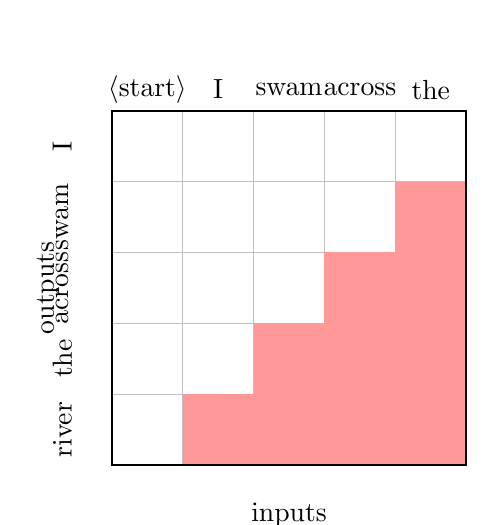
\begin{tikzpicture}[scale=0.9]
\draw[step=1cm, gray!50, very thin] (0,0) grid (5,5);
\foreach \x in {0,...,4} {
    \foreach \y in {0,...,4} {
        \ifnum\x>\y
            \fill[red!40] (\x,\y) rectangle (\x+1,\y+1);
        \fi
    }
}
\draw[thick] (0,0) rectangle (5,5);
\node[rotate=90] at (-0.9,2.5) {outputs};
\node at (2.5,-0.7) {inputs};
\node at (0.5,5.3) {$\langle\text{start}\rangle$};
\node at (1.5,5.3) {I};
\node at (2.5,5.3) {swam};
\node at (3.5,5.3) {across};
\node at (4.5,5.3) {the};
\node[rotate=90] at (-0.7,0.5) {river};
\node[rotate=90] at (-0.7,1.5) {the};
\node[rotate=90] at (-0.7,2.5) {across};
\node[rotate=90] at (-0.7,3.5) {swam};
\node[rotate=90] at (-0.7,4.5) {I};
\end{tikzpicture}
\end{center}

\subsubsection{Batching and Padding}

\begin{itemize}
    \item For efficient GPU utilization, multiple sequences are combined into an input tensor and processed in a single batch.
    \item Batching requires each sequence to have the same length, so shorter sequences are padded with a special $\langle\text{pad}\rangle$ token.
    \item A \textbf{padding mask} is added to the attention computation so that tokens representing real content never attend to padded positions.
\end{itemize}

\subsubsection{Using the Trained Decoder}

\begin{itemize}
    \item The model outputs a probability distribution over the vocabulary via the softmax layer, representing the likelihood of each possible next token given the current prefix.
    \item After sampling or selecting the next token, the extended sequence is fed back through the decoder to generate the subsequent token; this loop continues until an end-of-sequence token is produced.
    \item Thanks to masked attention, the representation of an existing token depends only on earlier tokens and therefore does not need to be recomputed when later tokens are generated, enabling reuse of intermediate activations.
\end{itemize}

\end{document}


% fino a 49 compresa 